\section{Experiments}
\label{sec:experiments}

We evaluate \method{} in two OPSD settings: (1) coding with rich environment feedback and (2) science reasoning without rich environment feedback. We compare against GRPO~\citep{shao2024deepseekmath} and SDPO~\citep{hubotter2026sdpo} in both settings, and additionally against TRD~\citep{jiang2026trajectory} on LiveCodeBench. These methods differ in how training trajectories are constructed: SDPO distills along the original student-generated trajectory, TRD distills along a teacher-regenerated trajectory, and \method{} distills along a student-regenerated trajectory initiated by a teacher-selected branch.







































































\subsection{Learning with Rich Environment Feedback}

\paragraph{Setup.}
We train Qwen3-8B, Qwen3-14B, and Olmo3-7B-Instruct on LiveCodeBench v6 with rich environment feedback. For each failed rollout, the privileged context is a successful sibling when available, and otherwise execution feedback from the verifier. We compare \method{} with GRPO, SDPO, and TRD over 80 training updates. We select the checkpoint with the highest Avg@4 and report Pass@4 from the same checkpoint. Appendix~\ref{app:lcb-hparams} provides the full experimental details.

\begin{table}[t]
  \caption{Best Avg@4 and corresponding Pass@4 (\%) within 80-step training on LiveCodeBench v6 with rich environment feedback. Bold and underlining mark the highest and second-highest trained-method values in each column.}
  \label{tab:lcb-results}
  \centering
  \small
  \setlength{\tabcolsep}{0pt}
  
  \begin{tabular*}{\linewidth}{@{\hspace{3pt}}p{\dimexpr0.20\linewidth-6pt\relax}*{8}{>{\centering\arraybackslash}p{0.101\linewidth}}@{}}
    \toprule
    Method & \multicolumn{2}{c}{Qwen3-8B} & \multicolumn{2}{c}{Qwen3-14B} & \multicolumn{2}{c}{Olmo3-7B-Instruct} & \multicolumn{2}{c}{Average} \\
    \cmidrule(lr){2-3} \cmidrule(lr){4-5} \cmidrule(lr){6-7} \cmidrule(lr){8-9}
    & Avg & Pass & Avg & Pass & Avg & Pass & Avg & Pass \\
    \midrule
    
    
    
    
    
    
    
    
    
    Base & 27.5 & 36.1 & 28.6 & 35.1 & 32.1 & 42.7 & 29.4 & 38.0 \\
    + GRPO & 40.7 & 44.0 & 44.1 & 48.1 & 39.3 & \underline{48.1} & 41.4 & 46.7 \\
    + SDPO & \underline{48.1} & \underline{48.6} & \underline{48.9} & \underline{48.9} & \underline{50.8} & \textbf{53.4} & \underline{49.2} & \underline{50.3} \\
    + TRD & 39.3 & 41.2 & 48.1 & 48.1 & 38.0 & 40.5 & 41.8 & 43.3 \\
    + \textbf{\method{}} (ours) & \textbf{49.2} & \textbf{49.6} & \textbf{51.1} & \textbf{51.1} & \textbf{51.0} & \textbf{53.4} & \textbf{50.4} & \textbf{51.4} \\
    \bottomrule
  \end{tabular*}
  \vspace{-0.1cm}

  
  
  
  
  
  
  
  
  
  
  
  
  
  
  
  
  
  
  
  
  
\end{table}

\vspace{-0.1cm}\paragraph{Results.}
Table~\ref{tab:lcb-results} shows that \method{} achieves the highest Avg@4 across all three models and the highest Pass@4, tying SDPO on Olmo3-7B-Instruct. Averaged across models, \method{} reaches $50.4\%$ Avg@4 and $51.4\%$ Pass@4, compared with $49.2\%$ and $50.3\%$ for SDPO. These gains show that, even with rich execution feedback and dense token-level supervision, performance improves when the teacher-preferred action is used to collect an alternative student continuation. Unlike SDPO, which distills along the original student suffix, \method{} supervises the student-generated continuation that follows the teacher-selected branch. This result supports trajectory collection as an additional design dimension for using privileged feedback effectively.


\subsection{Learning without Rich Environment Feedback}

\paragraph{Setup.}
We study SciKnowEval L3, which contains undergraduate-level biology, chemistry, materials science, and physics problems. Following SDPO~\citep{hubotter2026sdpo}, \method{} and SDPO use a successful sibling as privileged context for a failed rollout when one is available. We additionally compare with off-policy and on-policy GRPO. We exclude TRD from this setting because full-teacher regeneration exhibits severe training instability on SciKnowEval (Section~\ref{sec:method-student-generation}). Training is limited to 10 hours. We report both step-matched and time-matched comparisons, using Avg@128 for checkpoint selection and reporting Pass@128 from the same checkpoint. Table~\ref{tab:science-reasoning} reports performance across the four domains, and Appendix~\ref{app:science-hparams} provides the full experimental details.

\vspace{-0.1cm}\paragraph{Results.}
Table~\ref{tab:science-reasoning} shows that \method{} achieves the highest average Avg@128 under both the equal-step and equal-time comparisons. Averaged across the four domains, \method{} reaches 73.5\% under the 200-step budget and 74.5\% under the 10-hour budget, improving over SDPO by 0.8 and 0.3 percentage points, respectively. Together with the LiveCodeBench results, these gains show that teacher-guided branching can improve OPSD both with rich execution feedback and when privileged supervision is limited to successful sibling trajectories.

\begin{table}[t]
  \caption{Best Avg@128 (\%) on SciKnowEval L3 without rich environment feedback (Qwen3-8B). Steps and Hours denote training budgets of 200 steps and 10 hours, respectively. Average is the unweighted mean across the four disciplines. Bold and underlining mark the highest and second-highest means in each column among the reported methods.}
  \label{tab:science-reasoning}
  \centering
  \small
  \setlength{\tabcolsep}{3pt}
  
  
  
  
  
  
  
  
  
  \begin{tabular*}{\linewidth}{@{\hspace{6pt}\extracolsep{\fill}}l*{10}{c}@{\hspace{6pt}}}
    \toprule
    Method & \multicolumn{2}{c}{Biology} & \multicolumn{2}{c}{Chemistry} & \multicolumn{2}{c}{Materials} & \multicolumn{2}{c}{Physics} & \multicolumn{2}{c}{Average} \\
    \cmidrule(lr){2-3} \cmidrule(lr){4-5} \cmidrule(lr){6-7} \cmidrule(lr){8-9} \cmidrule(lr){10-11}
    & Steps & Hours & Steps & Hours & Steps & Hours & Steps & Hours & Steps & Hours \\
    \midrule
    Base & 30.6 & 30.6 & 41.6 & 41.6 & 59.0 & 59.0 & 59.0 & 59.0 & 47.6 & 47.6 \\
    + GRPO & \underline{59.6} & \underline{63.8} & 73.9 & 75.2 & \textbf{78.5} & \textbf{80.1} & 73.6 & 73.6 & 71.4 & 73.2 \\
    + GRPO (on-policy) & 51.5 & 51.5 & 66.8 & 66.8 & 73.4 & 73.4 & 69.4 & 69.4 & 65.2 & 65.2 \\
    + SDPO & 57.4 & 61.1 & \underline{79.5} & \textbf{81.1} & \underline{77.5} & \underline{78.1} & \underline{76.3} & \underline{76.3} & \underline{72.7} & \underline{74.2} \\
    
    + \textbf{\method{}} (ours) & \textbf{60.7} & \textbf{63.9} & \textbf{80.4} & \underline{80.8} & 74.7 & 75.1 & \textbf{78.2} & \textbf{78.3} & \textbf{73.5} & \textbf{74.5} \\
    
    
    
    
    
    
    
    
    \bottomrule
  \end{tabular*}
\end{table}




















\subsection{Additional Results}
\label{sec:additional-results}

















\paragraph{Performance across training data scale.}
We additionally compare Qwen3-8B training on LCB-Large, which combines v1--v6, and LCB-Small, which contains v6, to examine performance and learning efficiency across training data scales. Figure~\ref{fig:lcb-learning-curve} reports Avg@4 through 80 updates. On LCB-Large, \method{} reaches $57.3$ Avg@4 and $87.8$ Pass@4, compared with the best baseline values of $54.3$ Avg@4 from GRPO and $86.3$ Pass@4 from SDPO. On LCB-Small, \method{} reaches $66.5$ Avg@4 and $92.4$ Pass@4, compared with $65.5$ and $92.1$ for SDPO. TRD reaches $59.9$ Avg@4 on LCB-Small, while its best Avg@4 on LCB-Large ($45.4$) remains below the base model ($49.6$). \method{} reaches the best baseline performance after $33\%$ fewer updates on LCB-Large and $56\%$ fewer updates on LCB-Small.





























\begin{figure}[t]
  \centering
  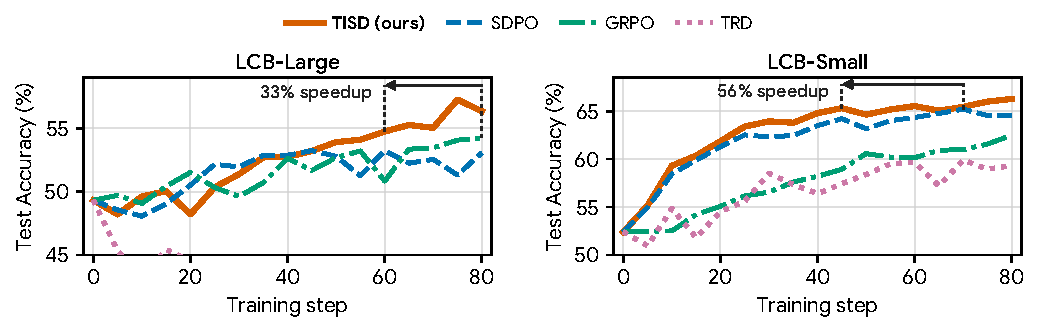
\includegraphics[width=\linewidth]{figures/lcb_large_small_mean_at_4.pdf}
  \vspace{-0.65cm}
  \caption{Mean test-case pass rate (Avg@4, \%) across training data scales, through 80 training steps in the rich-feedback setting (Qwen3-8B). LCB-Large combines v1--v6, and LCB-Small contains v6. \method{} first exceeds GRPO's maximum on LCB-Large with a $33\%$ speedup and reaches SDPO's maximum on LCB-Small with a $56\%$ speedup.}
  \label{fig:lcb-learning-curve}
  \vspace{-0.2cm}
\end{figure}

\vspace{-0.1cm}\paragraph{Does peak divergence identify a useful branch?}
The gains from regeneration depend on where the branch begins. We replace \method{}'s peak-divergence selector with either a uniformly random response position or the first student--teacher argmax disagreement, while keeping the remaining training and evaluation configuration fixed. On LCB-Small, peak-divergence branching reaches $66.5$ Avg@4, compared with $65.2$ for random-position branching and $64.6$ for first-disagreement branching (Figure~\ref{fig:lcb-branch-position-ablation}). Relative to SDPO at $65.5$ Avg@4, only peak-divergence branching improves performance among the evaluated selectors, supporting divergence magnitude as a useful criterion for selecting the branch position. Retaining the student's original token at the peak-divergence position and resampling the suffix (\emph{Student own token}) reaches only $64.8$ Avg@4, indicating that both the branch position and the teacher-selected action contribute to the gain.

A complementary diagnostic shows that the preferred intervention position depends on who generates the suffix. On failed Qwen3-8B LiveCodeBench v6 rollouts at initialization, forcing the teacher token and returning generation to the student succeeds more often at peak divergence than at the first argmax disagreement ($9.9\%$ vs.\ $6.1\%$). When the teacher instead generates the suffix, the first argmax disagreement yields higher success ($17.1\%$ vs.\ $13.3\%$; Appendix Table~\ref{tab:steer_qwen8b_positions}). Since \method{} returns suffix generation to the student, these results further support peak divergence as the branch selector for \method{}.



\vspace{-0.1cm}\paragraph{Is one regeneration sufficient?}
The standard procedure performs a single branch--regenerate operation. We additionally allow the regenerated trajectory to branch again at a strictly later position, while keeping the original privileged context fixed and making no additional verifier calls between rounds. Under the same 80-update schedule, two total rounds reach $65.2$ Avg@4 and $90.8$ Pass@4, while three rounds reach $65.5$ Avg@4 and $90.1$ Pass@4. In comparison, single-round regeneration achieves $66.5$ Avg@4 and $92.4$ Pass@4, the highest performance among the evaluated depths (Figure~\ref{fig:lcb-recursive-regeneration}). Thus, additional regeneration rounds do not improve performance under this fixed-feedback training setup, supporting the single-round design of \method{}.

\begin{figure}[t]
  \centering
  \begin{minipage}[t]{0.49\linewidth}
    \centering
    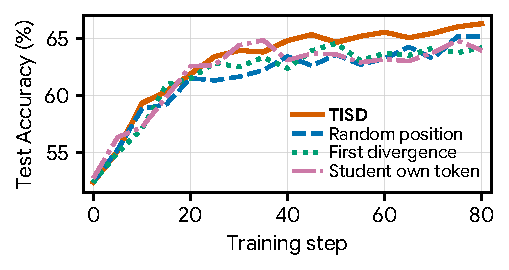
\includegraphics[width=\linewidth]{figures/lcb_branch_position_ablation.pdf}
  \vspace{-0.65cm}
\captionof{figure}{Branch-position and token ablations on Qwen3-8B LiveCodeBench v6 Avg@4 through update 80. Position controls use random positions or first argmax disagreement; Student own token retains the  token at peak reverse KL and resamples the suffix. }
    \label{fig:lcb-branch-position-ablation}
    
  \end{minipage}\hfill
  \begin{minipage}[t]{0.49\linewidth}
    \centering
    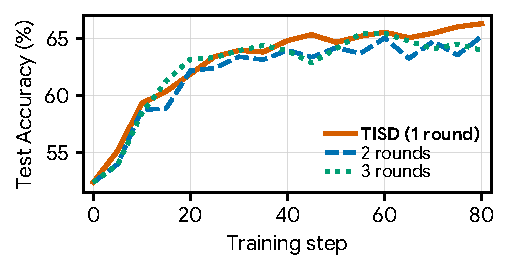
\includegraphics[width=\linewidth]{figures/lcb_recursive_regeneration.pdf}
  \vspace{-0.65cm}
\captionof{figure}{Effect of regeneration depth on Qwen3-8B LiveCodeBench v6 Avg@4 through update 80. Standard \method{} uses one branch--regenerate round; recursive variants apply two or three total rounds at strictly increasing response positions. }
    \label{fig:lcb-recursive-regeneration}
  \end{minipage}
  \vspace{-0.2cm}
\end{figure}











